\documentclass{article}
\usepackage[utf8]{inputenc}
\usepackage[T1]{fontenc}
\usepackage{graphicx}
\usepackage{hyperref}
\usepackage{geometry}
\geometry{margin=1in}

\title{ATHANASIA}
\date{Encyclopaedia Britannica (1771)}

\begin{document}
\maketitle

\section*{Historical source}
\textbf{Entry ID:} \texttt{entry-athanasia-2171} \\
\textbf{Volume ID:} 144850373 \\
\textbf{Character Count:} 1937

\subsection*{Extracted Text}
ATHANASIA, GOLDLOCKS, a genus of the polygania aqualia order, belonging to the fyngeneria class of plants. Of this genus, Dr.Limous mentions 11 \_Species\_ of which the followingic are by Mr Millerreckoned worthy of a place in those gardens where there are convenience for preferring tender plants, as some of the species will outlive the waters of this country. 1. The dentants grows naturally at the Cape of God Hope. It rises three or four feet high, finding out many fine branches garnished with pretty long narrow leaves, having form resemblance to thole of buckthown plannian. The branches are generally terminated by yellow flowers formed into a kind of tunnel. Thefe flowers appear early in summer, and the feeds ripen in autumn. 3. The trifectate is alio a native of Africa, as are the three following sorts. It is a damby plant, about the height of the former, fending out several weak shoots, garnished with awl-flagged until leaves let close to them, of a pale liberty onborn. The flowers are yellow, and terminate the branches in a corymbus. They appear in August, and the black ripen in Otolom. 3. The ethuthella rides with a strong flambaby halk to the heights of fic or eight feet, fending out many ligneous branches garnished with long narrow leaves terminating in four or five pairs like thole of fampiro. The flowers are like thole of the former, and appear in July and Au-guilt, being feduced by feeds which ripen in Otolber. 3. The pudeless hath frong woody flakes four or five feet high, covered with a woolly bark, as are alfo the branches, which are closely garnished with entire, fearshaped, woolly leaves, and are terminated by yel-low flowers hanging hang food,alks, and are sometimes fucceeded by feeds that ripen in the autumn. 5. The animals is a low annual plants, fellow rings above a foot, high, and feeding forth two or three lender branches garnished with wing-pointed leaves : the flalks are ter-minated



\section*{Source record}
\begin{itemize}
\item \textbf{Dataset:} \texttt{NationalLibraryOfScotland/encyclopaedia\_britannica\_illustrated}
\item \textbf{Dataset Revision:} \texttt{309f765b1ecc83e0a7f7762e44b4a927a7555443}
\item \textbf{Page ID:} \texttt{britannica:309f765b1ecc83e0a7f7762e44b4a927a7555443:train:2171} \\
  \textbf{Filename:} \texttt{page-2171-f8869fa95f19.jpg} \\
  \textbf{Row Index:} 2171 \\
  \textbf{SHA256:} \texttt{f8869fa95f190d0e...}
\end{itemize}

\begin{figure}[h]
\centering
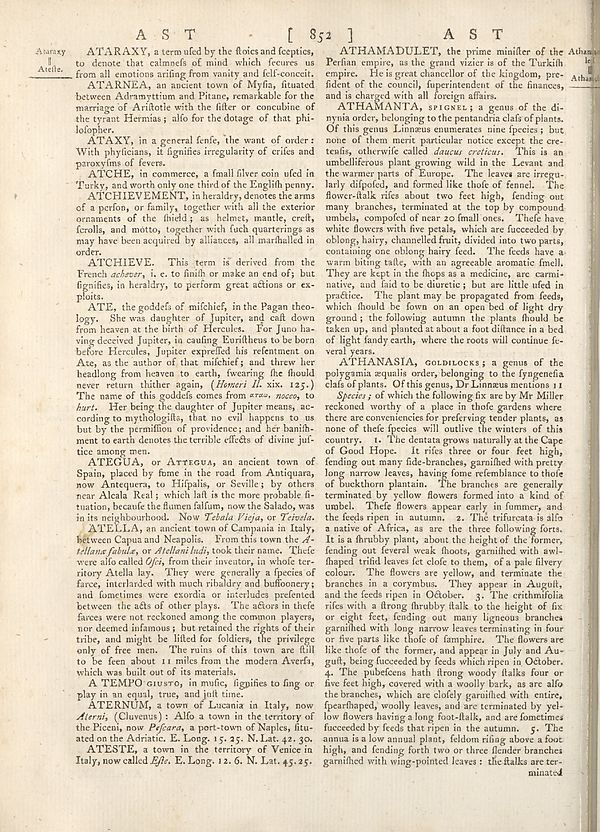
\includegraphics[width=0.85\textwidth]{../scans/page-2171-f8869fa95f19.jpg}
\caption*{Source scan: \texttt{page-2171-f8869fa95f19.jpg}}
\end{figure}

\end{document}
